This section discusses information regarding the initial time plan for the project, tollgates, activities, and the resources available. Throughout the project, work in a SCRUM-fashion is to be practiced. This is a technique well suitable for software development projects, and is a time efficient way of working. 

\begin{figure}[H]
\centering
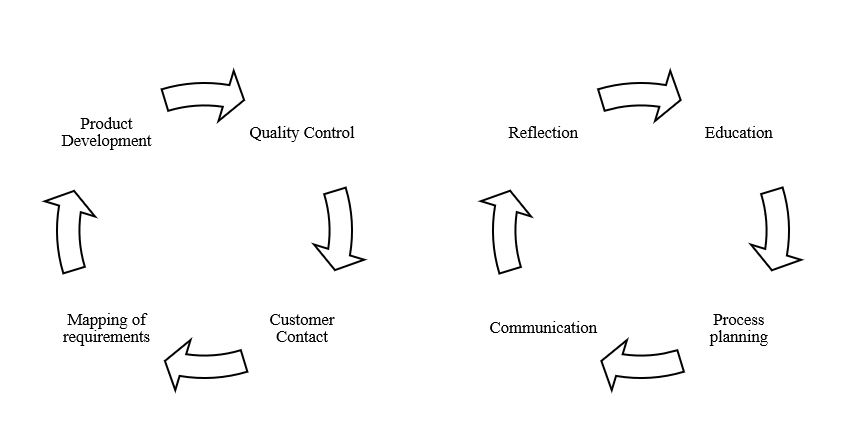
\includegraphics[width=\linewidth]{Pictures/processes.JPG}
\caption{Figure to show the intended way of working}
\label{fig:processes}
\end{figure}



\subsection{Deliverables}
Alongside the development of the software system and continuous delivery of the same, several supporting documents / artifacts are to be presented. These documents, like this project plan, is written to facilitate the development of a product in line with the customer requirements and available resources. The latest version of all these documents are to be found on the organisation platform Microsoft Teams. A list of these documents and explanation of its purpose is to be found below:
\begin{itemize}
    \item{\textbf{Project plan}} \\
    A document used to describe how the project is to be implemented as well for describing how testing and follow-up is to be done. 
    \item{\textbf{Software requirement specification, SRS}} \\
    Description of what requirements the customer has on the products that is to be delivered. The requirements are divided into functional and non-functional requirements and are also ranked regarding to it's importance for the system and customer. 
    \item{\textbf{Architecture notebook}} \\
    Description of how the architecture within the entire product / system is to be set up; how the database and front end is to be set up and how communication to external systems is implemented etcetera.  
    \item{\textbf{Test plan}} \\
    A document describing how the system is to be tested and how the documentation from the tests is to be maintained and stored. 
    \item{\textbf{Education plan}} \\
    How do we assure that the project organisation has the suitable knowledges for the different tasks? The education plan is set up to answer this question, meaning that the education plan is to be seen as a blueprint of how different knowledge needed within the project is to be acquired. 
    \item{\textbf{Software Quality Assurance, SQA}} \\
    Document describing how we are to assure a suitable quality on the product as well as for the processes implemented during the project. 
    \item{\textbf{Future Development}} \\
    Document to be developed in the end of the project. This document is to describe how the product is to be further developed after termination of the project. 
\end{itemize}
\subsection{Time and resource plan}
As mentioned in section 2.2, HeartByte has 160 hours per employee as a budget in this project. Apart from human resources, there's also knowledge resources. These resources are to be further developed if needed, see the education plan for further information. If needed, HeartByte is also able to consult other companies within the same industry to develop knowledge or program-modules.Regarding time plan, the project is divided into five different iterations - please see the figure below. 

\begin{figure}[H]
\centering
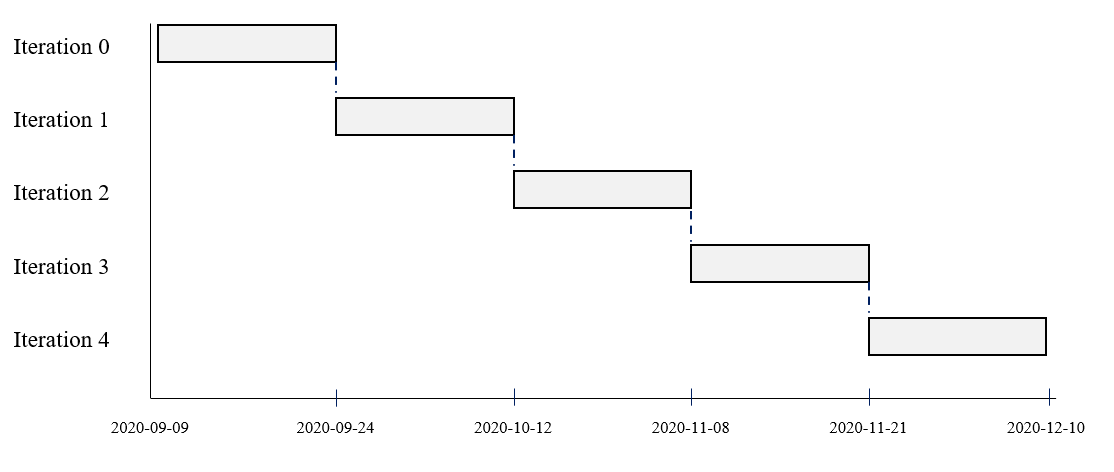
\includegraphics[width=\linewidth]{Pictures/all_iterations.jpeg}
\caption{Gantt-chart over planned iterations}
\label{fig:all_iterations}
\end{figure}
   
\subsubsection{Iteration 0}
Iteration 0, the pre-study phase, is a time where the organisation is to get to know the customer and its needs.The main focus lies in understanding what value the system has to create and how this could be done. The organisation pursues workshops regarding how this expected value creation can take place and how the product should be designed.

\begin{figure}[H]
\centering
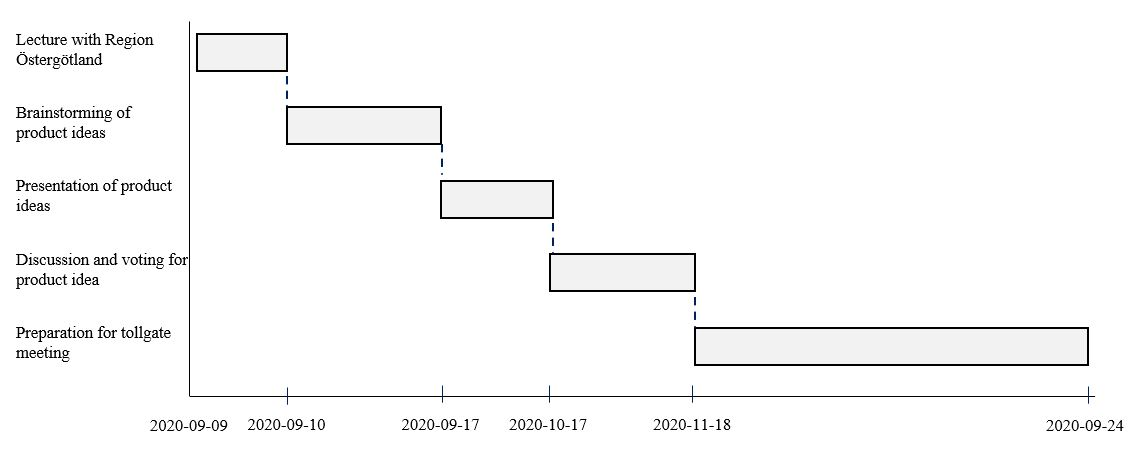
\includegraphics[width=\linewidth]{Pictures/iteration_0.JPG}
\caption{Gantt-chart over iteration 0}
\label{fig:iteration_0}
\end{figure}

The pre-study phase ends with a tollgate meeting where HeartByte is to present the results of the studies made. The customer is to decide if they support further development of the proposed product or if changes are needed.

\subsubsection{Iteration 1}
The processes taking place in iteration 1 are to be seen in the list below.
\begin{itemize}
    \item Map requirements for the product and get them accepted by the customer.
    \item Education within the organisation is to be initiated in order to develop the needed skills. According to the architecture notebook, the product is to be developed in React. Therefore, education within this language is to be pursued. For more information on this topic, please see the education plan. 
    \item Tests are to be planned and introduced starting off with lo-fi tests pursued with a lo-fi prototype.  The main goal with lo-fi testing is to get comments from intended users if the product is functional or not, or if there are any major aspects that has to be re-designed. For more information on this topic, see the test plan. 
     \item A CI environment is to be set up in order to enable continuous integration and development.
    \item A first version of the product is to be deployed and available for stakeholders to interact with. This puts a constraint on our development environment; before HeartByte is able to have a functional web site online, a working CI pipeline is required. 
    \item In order to be able to start coding the product, the initial list of requirements has to be accepted by the customer.
\end{itemize}


\begin{figure}[H]
\centering
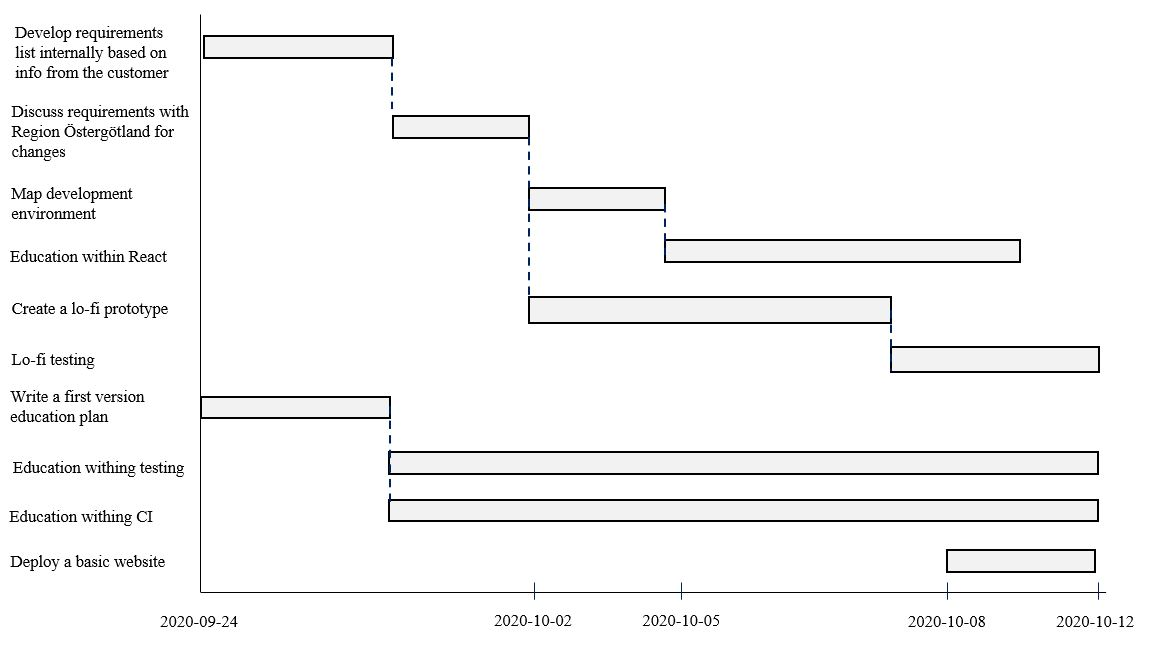
\includegraphics[width=\linewidth]{Pictures/iteration_1.JPG}
\caption{Gantt-chart over iteration 1}
\label{fig:iteration_1}
\end{figure}
 

\subsubsection{Iteration 2}
Iteration 2 holds two weeks of effective working time. See the list below for a summary of processes pursued:

\begin{itemize}
    \item The main focus for this iteration is to continue the development of components to the product: a main / home dashboard is to be developed according to the prototype as well as a patient list module. See the Lo-Fi prototype for more information.
    \item Unit tests are to be planned and developed for the modules integrated to the product so far.
    \item A Hi-Fi prototype is to be developed in Figma. This prototype is to serve as a blueprint for the developers when coding the product. The Hi-Fi prototype also enables more proper testing with intended end-users
\end{itemize} 

\begin{figure}[H]
\centering
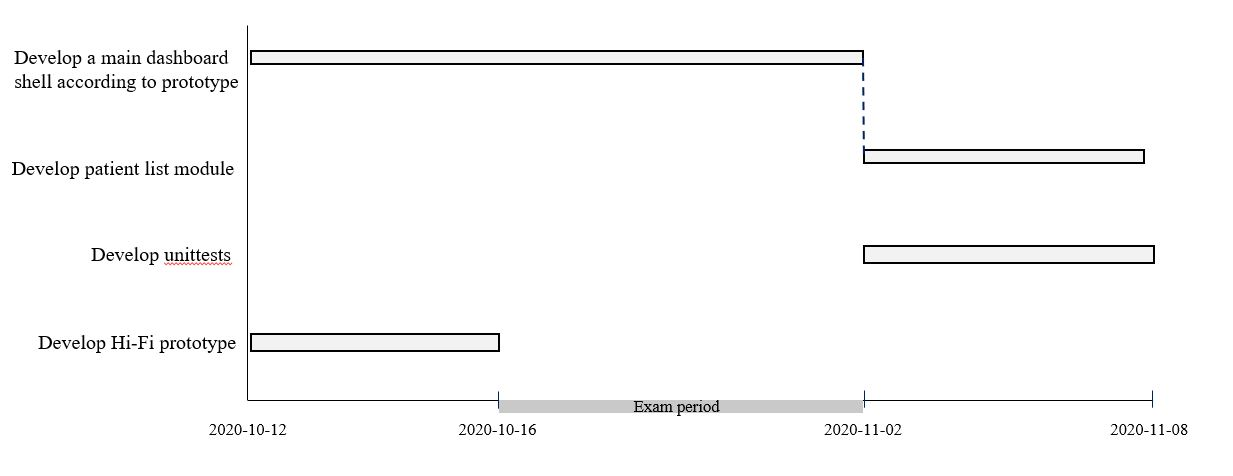
\includegraphics[width=\linewidth]{Pictures/iteration_2.JPG}
\caption{Gantt-chart over iteration 2}
\label{fig:iteration_2}
\end{figure}

\subsubsection{Iteration 3}

Iteration 3 spans over 2 weeks of time from 2020-11-08 to 2020-11-21. The main focus during these weeks is to review the processes intended to be used and to have been used in the project, as well as development of the product. See the list below for a summary of processes pursued:

\begin{itemize}
    \item Automated tests using Selenium are to be developed. For a detailed description of this process, see the test plan.
    \item The components developed for the product are to be continuously checked by our analysts make sure they meet the requirements. For more information regarding this process, see the SRS-document and the process-plan. 
    \item Possibilities for admin customization are to be developed and merged into the product. 
    \item Data fetching from the server is to be developed. 
    \item The rule engine regarding what data that is to be displayed in a certain state is to be developed.
    \item The personal database is to be further developed and finished. 
    \item User authentication is to be developed implemented into the product. 
    \item A notice board is to be developed and implemented.
    
\end{itemize} 

\begin{figure}[H]
\centering
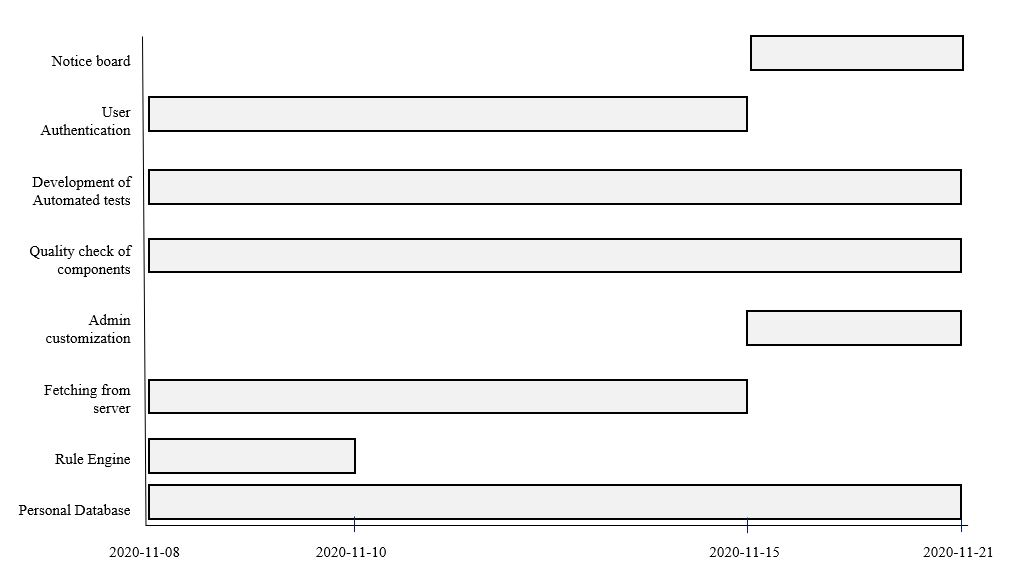
\includegraphics[width=\linewidth]{Pictures/iteration_3.JPG}
\caption{Gantt-chart over iteration 3}
\label{fig:iteration_3}
\end{figure}
 

\subsubsection{Iteration 4}
Iteration 4 stretches from 2020-11-21 until 2020-12-10. In this iteration, development is planned to take place until 2020-12-04 which is the date set for code stop. During this two weeks period of time, the main focus on the development side is to finish already ongoing tasks. This time is to be seen as buffer time. For a description of processes concerning the project as a whole, see the list below:
\begin{itemize}
    \item The development of the product is to be finished. 
    \item User tests with intended end-users are to be performed.
    \item Processes used in the project are to be updated regarding its documentation. 
    \item System \& integration tests are to be developed. See the test plan for detailed description.
    \item The delivery of the final product is to be planned and pursued. 
\end{itemize}

\begin{figure}[H]
\centering
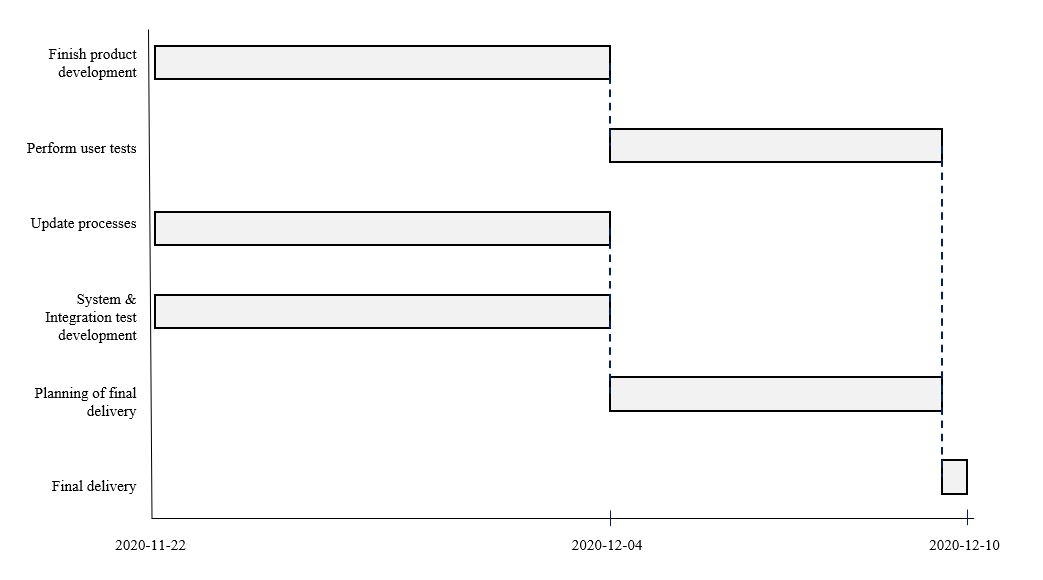
\includegraphics[width=\linewidth]{Pictures/iteration_4.JPG}
\caption{Gantt-chart over iteration 4}
\label{fig:iteration_4}
\end{figure}

\subsubsection{Development tasks summarized}
A more detailed list of the development tasks described in the iteration plan above is to be found below. The intention for these two lists is to describe the different tasks and sub tasks in a more thorough way than done in the iteration plan. The tasks are divided between front-end and back-end, and is to be seen as a complement to development tasks described in the iteration plan.  
\begin{figure}[hbt!]
\centering
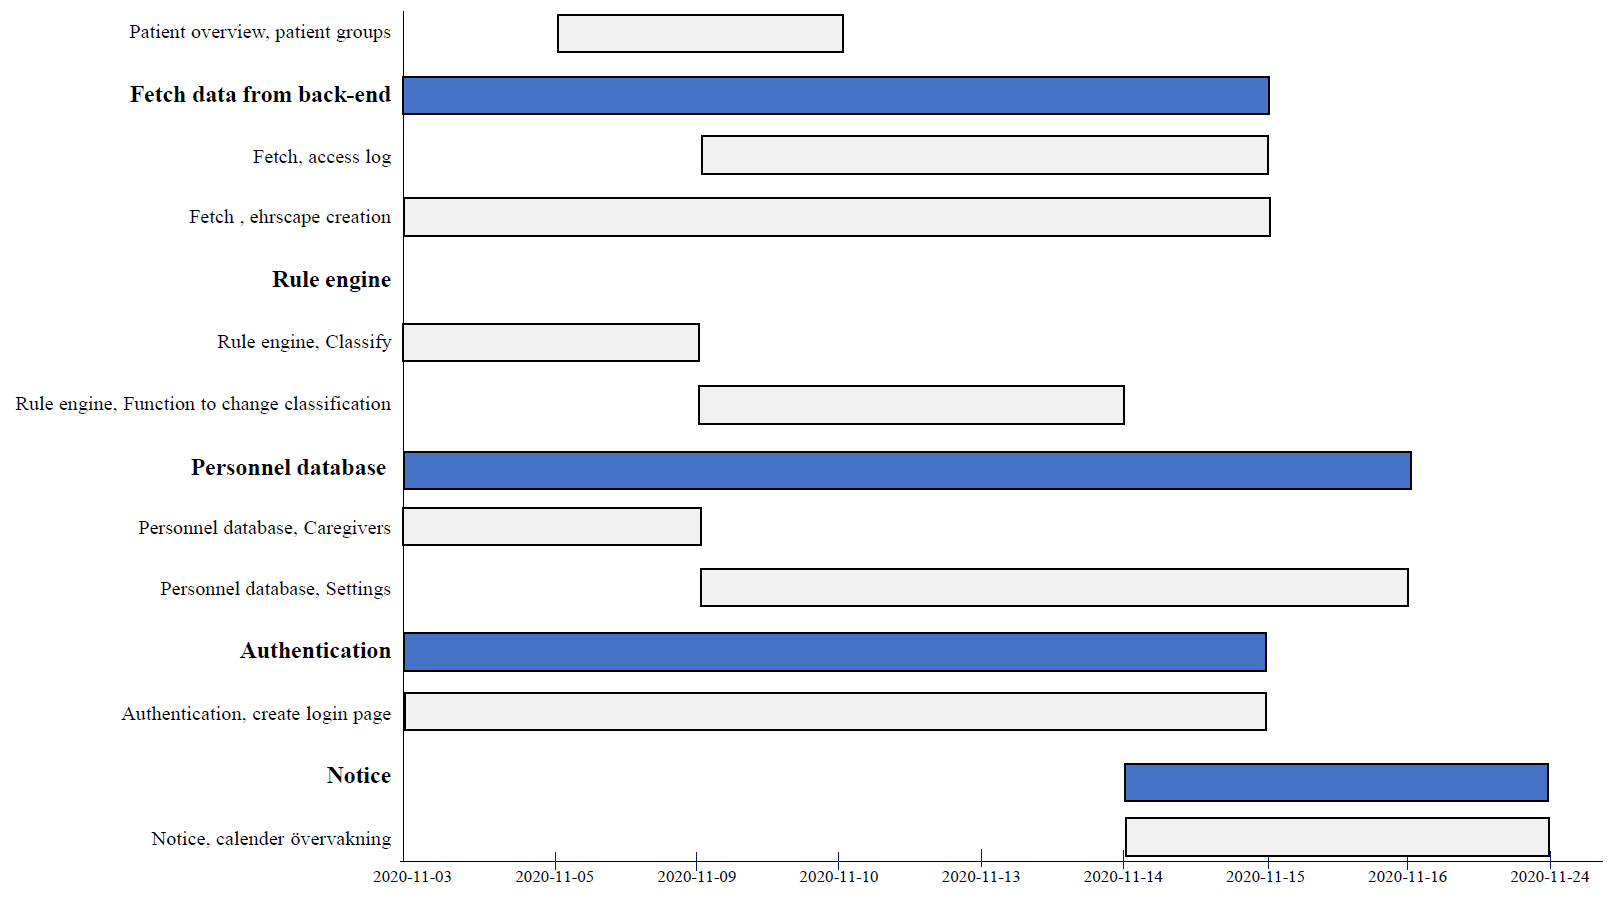
\includegraphics[width=\linewidth]{Pictures/DevTasksBackend.PNG}
\caption{Gantt-chart over planned tasks for the backend}
\label{fig:backend}
\end{figure}
\begin{figure}[hbt!]
\centering
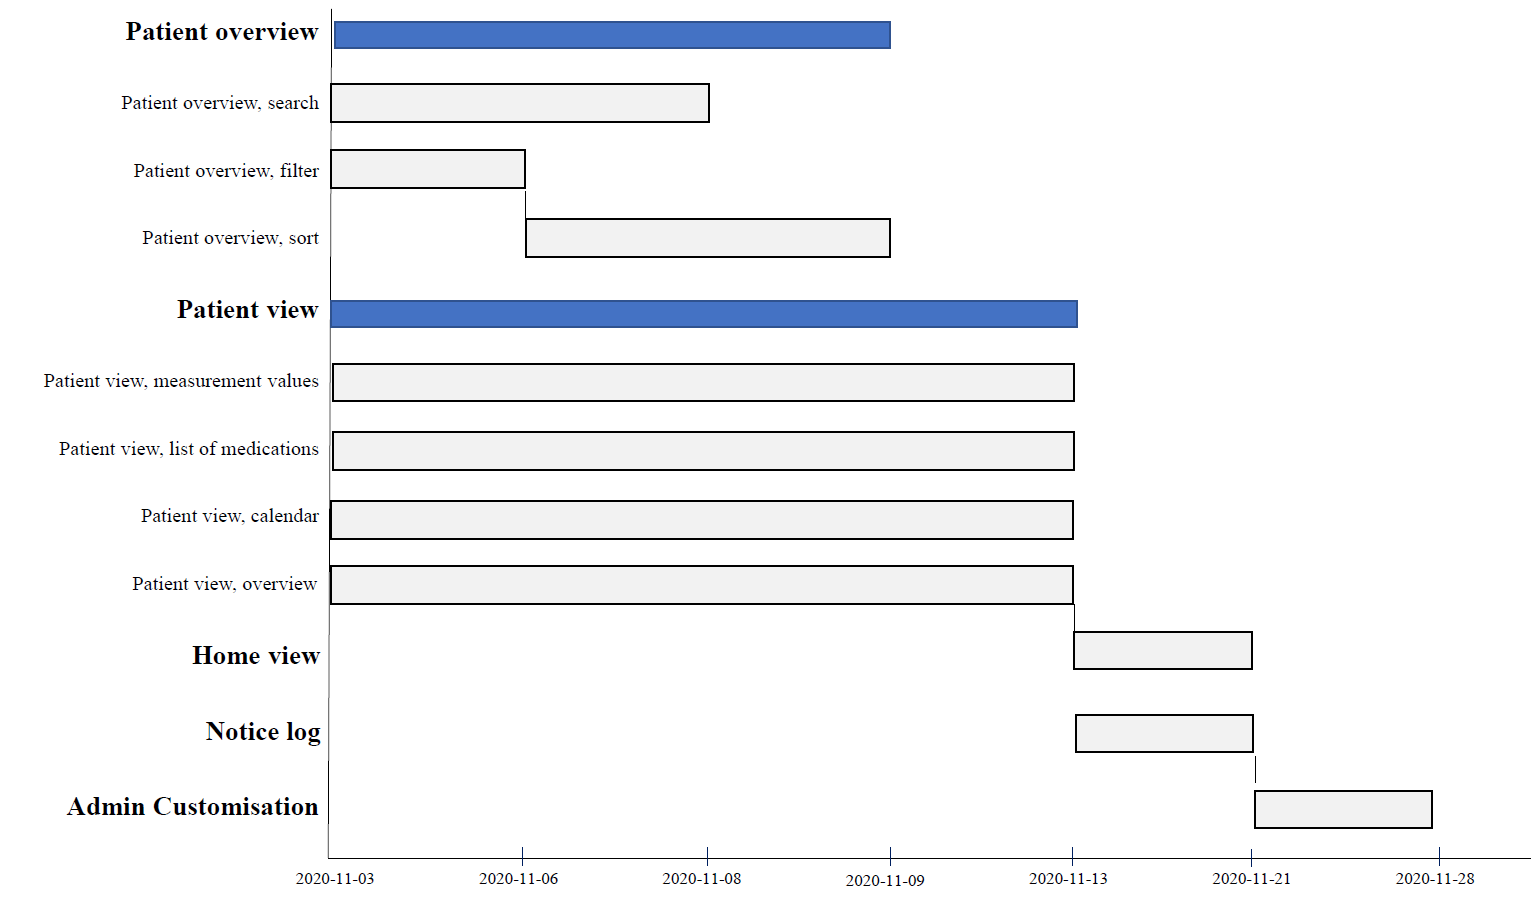
\includegraphics[width=\linewidth]{Pictures/DevTasksFrontend.PNG}
\caption{Gantt-chart over planned tasks for the frontend}
\label{fig:fronten}
\end{figure}

\newpage
\subsection{Tollgates}
A list of the defined tollgates is shown below, and is to be seen as a complement to the iteration plan.
\begin{itemize}
    \item 2020-09-24 - Tollgate meeting with Region Östergötland\\ \\
    This meeting is about approval from the customer that the idea for a product solution creates the value needed for the customer. Before the meeting with the customer and external stakeholders is held, the entire organization for the project gathers to pursue a preparation meeting. The material provided from the management team to be presented on the tollgate meeting with the customer is discussed. The main purpose of this meeting is to give the entire project team a possibility to comment on the material being presented for our customer. Doing so, everyone can come up with changes in the material if they find that the management team is lacking in any circumstances when describing the pre-study phase. \\
    
    \textit{Update: When this meeting was held, some minor comments were brought to the table by team members not being a part of the management group. The changes were implemented in the material to be presented for the customer before the main tollgate meeting.} 
    \item 2020-10-12 - Basic CI-pipeline set up and an initial web application launched\\ \\
    The CI-pipeline has to be developed in order to enable a first version of the web application to be launched. This version of the web application is to be very simple. 
    \item 2020-10-14 - Development tasks \& responsibilities handed out \\ \\
    Since the product is to be developed in React, the entire product will be divided into different components. The components are divided between smaller groups of developers in orders to create an effective workflow.
    \item 2020-11-08 - A functional dashboard developed \\ \\
    The system has a dashboard where the user can press the buttons to enter a patient modal to retrieve information about the specific patient. 
    \item 2020-12-04 - Code stop for developing the product\\ \\
    Friday the 4th of December is the last day where it's allowed to push new code to the project. The remaining time until delivery is time needed for last fixes of the delivery and deployment.
    \item 2020-12-10 - VSSE, the final presentation of the product\\ \\
    At this date the development of the product has to be fully terminated. The product has to be ready for delivery to the customer. 
\end{itemize}   

\begin{figure}[H]
\centering
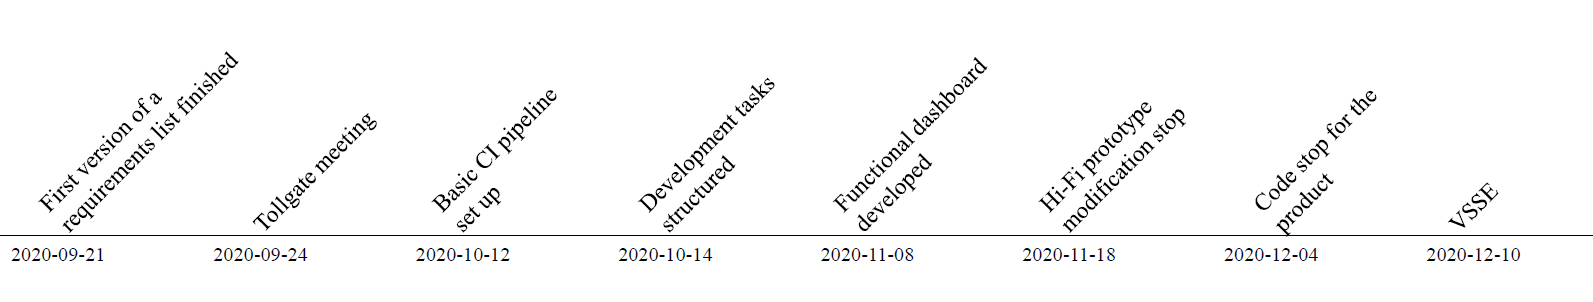
\includegraphics[width=\linewidth]{Pictures/timeline.PNG}
\caption{Timeline for what tollgates and deadlines the project is following}
\label{fig:timeline}
\end{figure}


\subsection{Activities}
Below are a brief description of the main activities being implemented in the project and their intended outcome / meaning. For a more thorough explanation, see the process-plan document 
\begin{itemize}
    \item{\textbf{Workshops}} \\
    Used to get the different teams within the organisation together to discuss future tasks and ideas. Workshops are to be planned several times during the project with different plans for each occasion. 
    \item{\textbf{Company meetings}} \\
    Meetings every Thursday where the entire company is brought together. Mostly used to discuss questions brought to the table by our external stakeholders or to discuss strategic matters for the project. 
    \item{\textbf{Mapping of requirements}} \\
    A process that is to be pursued together with the customer by our analyst team. The main reason for this task is to understand the many needs that our customer has and what requirements the product has to fulfill. 
    \item{\textbf{Development of Lo-Fi prototype}} \\
    A prototype firstly developed on paper without any functionalities. The main purpose for this prototype is to enable initial user testing as well as serve as a blueprint for the initial development / coding. 
    \item{\textbf{Writing of supporting documents}} \\
    The different documents mentioned above are written in order to enhance the performance for the entire company while working with the project in different ways. 
    \item{\textbf{Lo-Fi testing}} \\
    Tests performed with the lo-fi prototype together with our intended end-users. The reason for this process being implemented is to get some initial comments on any eventual clear mistakes done in the first design phase. 
    \item{\textbf{Planning of education}} \\
    In order to be able to develop the product ordered by the customer, education has to be performed in a structured manner for the applicable sub-teams within the company. Therefore, writing an education plan is essential. 
    \item{\textbf{Mapping of requirements}} \\
    The team has to realize how the requirements stated by the customer is to be taken in consideration in the development process. 
    \item{\textbf{Development}} \\
    The actual coding / development of the product. This process is broken down into several sub-tasks and pursued in a SCRUM-manner. 
    
    \item{\textbf{Testing}} \\
    Only performing lo-fi testing with our lo-fi prototype is not enough in order to ensure the customer that the product meets their requirements. Therefore, continuous unit- and web testing is required though out the development process. 

\end{itemize}






